%% Warm-up paper: document classes and the packages academic templates use,
%% including bibliography, hyperlinks and figure insertion.
\documentclass[11pt]{article}
\usepackage{agentikz-fonts}
\usepackage[a4paper,margin=2.5cm]{geometry}
\usepackage{amsmath,mathtools,amssymb,bm}
\usepackage{graphicx}
\usepackage{booktabs}
\usepackage{algorithm}
\usepackage{algpseudocode}
\usepackage{caption,subcaption}
\usepackage{hyperref}
\usepackage{natbib}
\usepackage{tikz}
\usepackage{pgfplots}
\pgfplotsset{compat=1.18}
\begin{document}
\section{引言 Introduction}
中英混排正文与公式 $E=mc^2$，引用 \citep{agentikz}.
\begin{center}
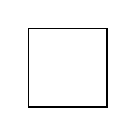
\begin{tikzpicture}\draw (0,0) rectangle (1,1);\end{tikzpicture}
\end{center}
\bibliographystyle{plainnat}
\end{document}
